% !TEX root = ../main.tex
% !TEX spellcheck = en_GB

\chapter{Requirements}

In this chapter the requirements for the system will be described.
In total four use cases have been defined, which describe the functionality and the actor's interaction with the \systemName system.
These use cases establish the foundation of the requirements specification.

\begin{figure}[H]
	\centering
	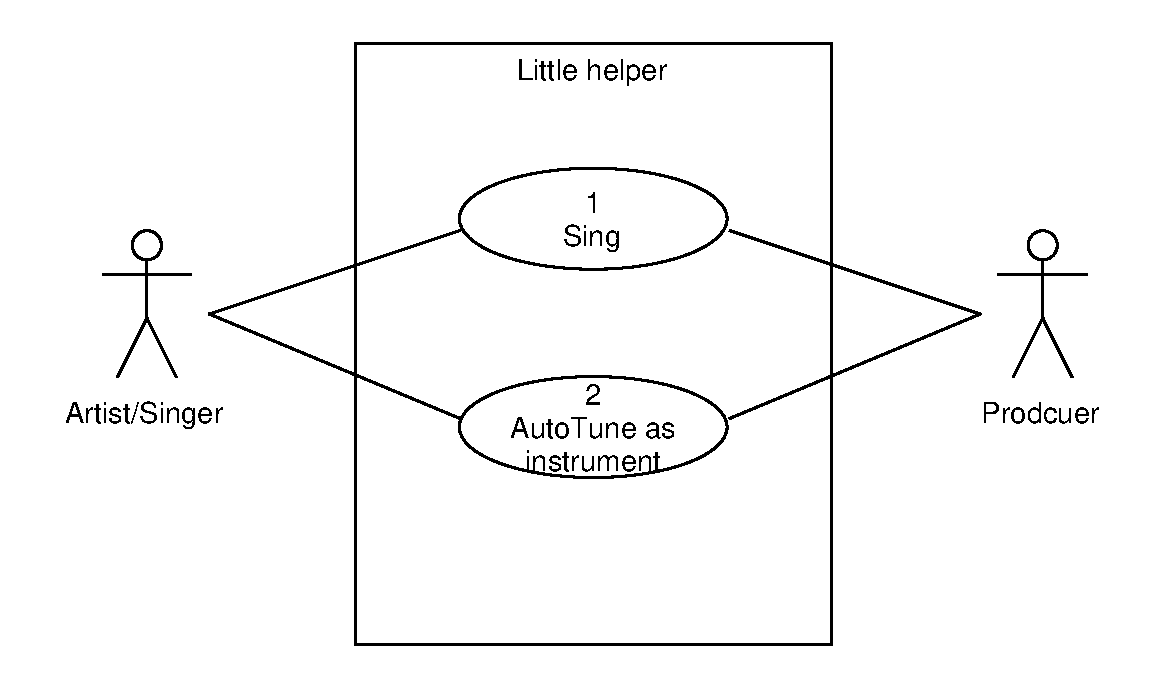
\includegraphics[width=0.7\linewidth]{Design/UseCaseDiagram.pdf}
	\caption{Use Case diagram.}
	\label{fig:UCDiagram}
\end{figure}

\section{Actor descriptions}

\begin{table}[H]
	\centering
	\begin{tabularx}{\textwidth}{p{0.2\textwidth} X}
		\toprule
		\textbf{Name of actor} & Artist \\
		\textbf{Type} & Primary \\
		\textbf{Description} & Is a live performer.
		The goal for the Artist can be either to be corrected into perfect pitch (e.g. from \SI{443}{\hertz} to \SI{440}{\hertz}), or to create the robotic sound often associated with auto tune (e.g. Cher - Believe). \\
		\bottomrule
	\end{tabularx}
	\caption{Actor description of Artist.}
	\label{tab:actorArtist}
\end{table}

\begin{table}[H]
	\centering
	\begin{tabularx}{\textwidth}{p{0.2\textwidth} X}
		\toprule
		\textbf{Name of actor} & Producer \\
		\textbf{Type} & Primary \\
		\textbf{Description} & Decides how the sounds are during recordings. The producer needs to be able to change the amount of auto tuning used during the recording, to find the right balance. \\
		\bottomrule
	\end{tabularx}
	\caption{Actor description of Producer.}
	\label{tab:actorProducer}
\end{table}

\begin{table}[H]
	\centering
	\begin{tabularx}{\textwidth}{p{0.2\textwidth} X}
		\toprule
		\textbf{Name of actor} & Audience \\
		\textbf{Type} & Secondary \\
		\textbf{Description} & The recipient of the live performance or studio recording. Is interested in hearing the music as the Artist/Producer intended it to be heard. \\
		\bottomrule
	\end{tabularx}
	\caption{Actor description of Audience.}
	\label{tab:actorAudience}
\end{table}

\section{Use Cases}
\label{rap:UC}
\Cref{fig:UCDiagram} shows the defined use cases and the different actors involved in each of them.

\subsection{Use Case 1 - Pitch correction}
\begin{table}[H]
	\centering
	\begin{tabularx}{\textwidth}{p{0.3\textwidth} X}
		\toprule
		\textbf{Name} & Pitch correction \\
		\midrule
		\textbf{Goal} & To move an off tune sound onto a piano scale tune. \\
		\midrule
		\textbf{Initiation} & Singing commences.\\
		\midrule
		\textbf{Actors and Stakeholders} & Artist, Producer and Audience. \\
		\midrule
		\textbf{References} & \\
		\midrule
		\textbf{Number of concurrent occurrences} & 1 \\
		\midrule
		\textbf{Precondition} & Resolution and scale is set. \\
		\midrule
		\textbf{Post-condition} & Output sound is moved to the nearest on-pitch frequency, determined by the resolution and scale. \\
		\midrule
		\textbf{Main scenario} & 
		\begin{enumerate}[noitemsep, topsep=0pt]
			\item Artist starts singing off pitch.
			\item Artist/Producer engages Pitch correction.
			\item[\textbf{EXT1}]
			\item Output sound is on pitch according to the set resolution.
		\end{enumerate}
		\\
		\midrule
		\textbf{Extension} & 
		\textbf{EXT1}
		\begin{enumerate}[noitemsep, topsep=0pt]
			\setcounter{enumi}{2}
			\item Sound is not as Artist/Producer wants it.
			\item Artist/Producer changes resolution or scale.
		\end{enumerate}
		\\
		\midrule
		\textbf{Data Variations List} & \\
		\bottomrule
	\end{tabularx}
\end{table}
\fxnote{What is meant with resolution?}
